\documentclass[margin=3pt,
  convert,
  convert={
    outext=.png,
    command=\unexpanded{
      pdftocairo -r 300 -png \infile % 将生成的pdf文件转换为png图像
    }
  }
  ]{standalone}

\usepackage{tkz-euclide}

\begin{document}

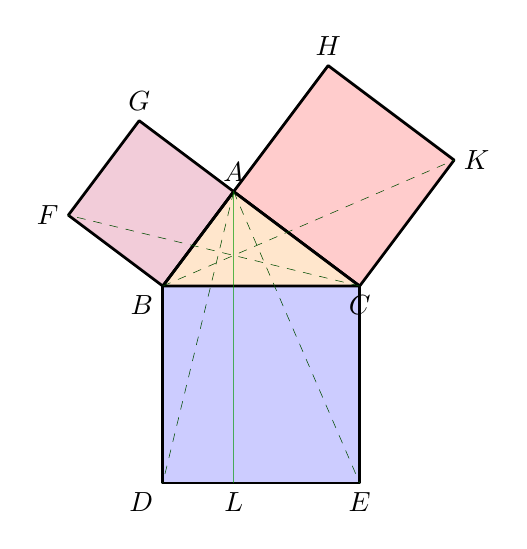
\begin{tikzpicture}[scale=.5]
  \tkzInit
  % 用坐标直接定义B、C点
  \tkzDefPoint(0,0){B}
  \tkzDefPoint(5,0){C}
  % 以B点为圆心半径为3和以C点为圆心半径为4的两个圆的交点为A点
  \tkzInterCC[R](B, 3 cm)(C, 4 cm)\tkzGetPoints{A}{A'}
  % 定义矩形
  \tkzDefSquare(B,A)\tkzGetPoints{G}{F}
  \tkzDefSquare(A,C)\tkzGetPoints{K}{H}
  \tkzDefSquare(C,B)\tkzGetPoints{D}{E}
  % 定义过A的垂线与DE的交点
  \tkzDefPointBy[projection = onto D--E](A) \tkzGetPoint{L}
  % 绘制填充多边形
  \tkzFillPolygon[fill = red!20 ](A,C,K,H)
  \tkzFillPolygon[fill = blue!20 ](C,B,D,E)
  \tkzFillPolygon[fill = purple!20](B,A,G,F)
  \tkzFillPolygon[fill = orange,opacity=.2](A,B,C)
  % 绘制多边形
  \tkzDrawPolygon[line width = 1pt](A,B,C)
  \tkzDrawPolygon[line width = 1pt](A,C,K,H)
  \tkzDrawPolygon[line width = 1pt](C,B,D,E)
  \tkzDrawPolygon[line width = 1pt](B,A,G,F)
  % 绘制指定线段
  \tkzDrawSegment[green!60!black](A,L)
  \tkzDrawSegment[dashed, green!30!black](A,D)
  \tkzDrawSegment[dashed, green!30!black](A,E)
  \tkzDrawSegment[dashed, green!30!black](C,F)
  \tkzDrawSegment[dashed, green!30!black](B,K)
  % 绘制各点的标记
  \tkzLabelPoints[above](A)
  \tkzLabelPoints[below left](B)
  \tkzLabelPoints[below left](D)
  \tkzLabelPoints[below](L)
  \tkzLabelPoints[left](F)
  \tkzLabelPoints[above](G)
  \tkzLabelPoints[above](H)
  \tkzLabelPoints[right](K)
  \tkzLabelPoints(C,E)
\end{tikzpicture}

\end{document}

%%% Local Variables:
%%% mode: latex
%%% TeX-master: t
%%% End:
